\documentclass[11pt]{exam}
\usepackage{epsfig}

\usepackage{hyperref}

\usepackage[centertags]{amsmath}
%\usepackage{amsfonts}
\usepackage{amssymb}
\usepackage{bbm}
\usepackage{amsthm}
\usepackage[all]{xy}
\usepackage{newlfont}
\usepackage{amsmath,amssymb,bm,mathtools}

\usepackage{xcolor} %for color
\usepackage{xmpmulti}
%\usetheme{Air}
%\usefonttheme{professionalfonts}
\usepackage{thumbpdf}
\usepackage{wasysym}
\usepackage{upgreek}

\usepackage{ucs}
%\usepackage[utf8]{inputenc}
\usepackage{pgf,pgfarrows,pgfnodes,pgfautomata,pgfheaps,pgfshade}
\usepackage{verbatim}
\usepackage{empheq}
\newcommand*\widefbox[1]{\fbox{\hspace{2em}#1\hspace{2em}}}

\newcommand{\Integer}{\mathbb{Z}}
\newcommand{\Natural}{\mathbb{Z}_{\geq 0}}
\newcommand{\Naturalstar}{\mathbb{Z}_{> 0}}
\newcommand{\Real}{\mathbb{R}}
\newcommand{\Complex}{\mathbb{C}}
\newcommand{\hilbert}{\mathcal{H}}
\newcommand{\BigHilbert}{\bm{\mathcal{H}}}
\newcommand{\innprod}[2]{\langle{#1},{#2}\rangle}
\newcommand{\ginnprod}[2]{\langle\!\langle{#1},{#2}\rangle\!\rangle}
\newcommand{\norm}[1]{\|{#1}\|}
\newcommand{\mrm}[1]{{\mathrm #1}}
\newcommand{\gnorm}[1]{|\!|\!|{#1}|\!|\!|}
\newcommand{\expect}{\mathbb{E}}

\newcommand{\gr}{\selectlanguage{greek}}

\setcounter{MaxMatrixCols}{20}

\begin{document}
\centerline{\Large \sc Homework 3}
\pagestyle{empty}

\hrulefill

\vspace{2cm}


{\Large \sc Name:}



\vspace{2cm}



{\Large \sc Student ID: }

\vspace{6cm}

\begin{itemize}
  \item Reasoning and work must be shown to gain partial/full
  credit
  \item Please include the cover-page on your homework PDF with your name and student ID. Failure of doing so is considered bad citizenship. 

 \end{itemize}

\clearpage
%{\bf Homework instructions}: You need to solve either question 1 or question 2, and you need to solve question 3. The homework total score will be the average given to two questions, either question 1 or 2, and that of question 3. You can solve the three questions if you wish; in that case of the two I will chose the one that has the highest score. 

\begin{questions}
\question[1--4]{\bf Algebra of graphs}:
Considering the undirected graph in the figure, do the following:
\begin{center}
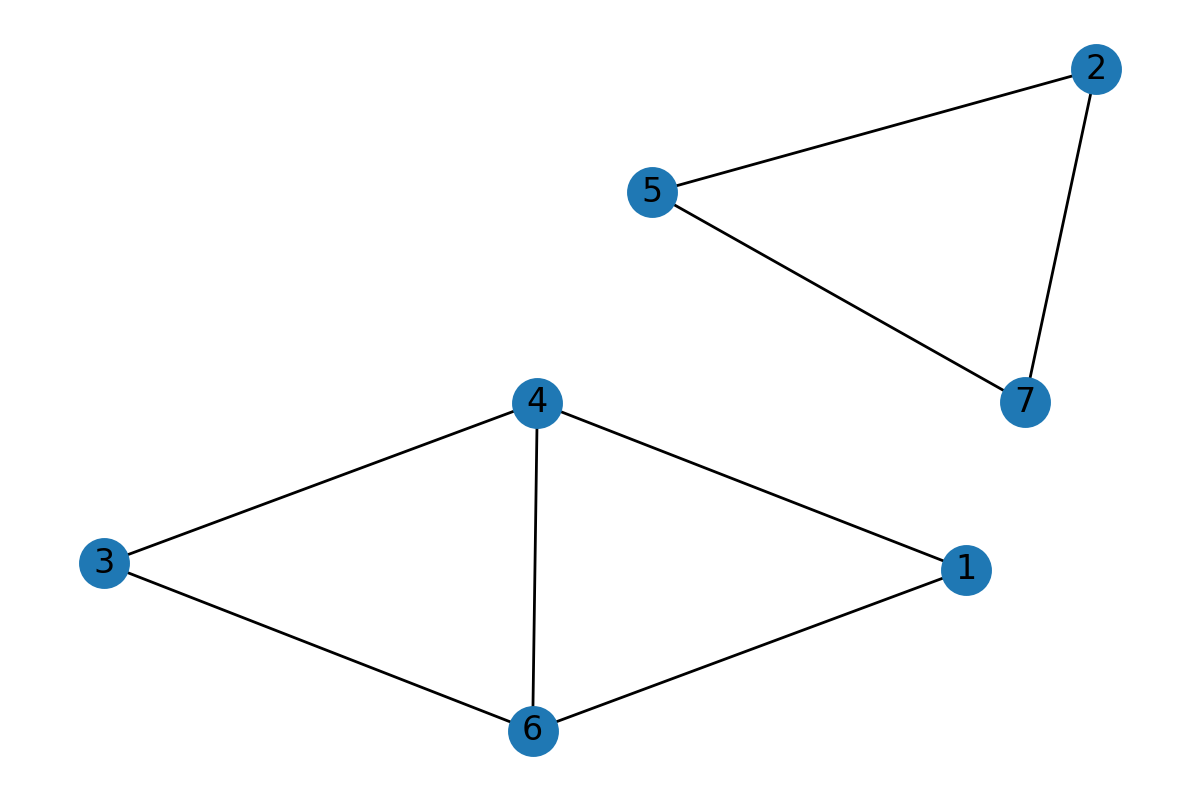
\includegraphics[width=0.4\linewidth]{homework3.png}
\end{center}
\begin{parts}
%Reorder nodes so that it doesn't look block diagonal.
\part Write the adjacency matrix of the graph \\
\part Then, write both the directed (oriented) and undirected (unoriented) incidence matrix of the graph. (\textit{Hint: For the directed incidence matrix, pick a random direction for each edge.})  \\

\part Verify in networkx that the Laplacian matrix of the graph is $\mathbf{L} = \mathbf{D} - \mathbf{A}$ where $\mathbf{D} = \text{diag}\left(\mathbf{d}\right)$ and $\mathbf{d}$ is a vector containing the degree of each node, and $\mathbf{A}$ is the adjancency matrix of the graph. Also, verify that $\mathbf{L} = \mathbf{B}\mathbf{B}^T$ where $\mathbf{B}$ is the \underline{directed} incidence matrix. \\
\part Show that there exist two linearly independent vectors that are in the null-space of the Laplacian and explain why that is the case.  \\
\end{parts}

\question[1--4]{\bf Graphs with circular symmetry}: Consider an undirected graph with circular symmetry, that is a graph ${\cal G}=({\cal V}, {\cal E})$ where
${\cal V}=\{0,\ldots, N-1\}$ is the set of nodes and $\mathcal{E} = \{e_0,e_1,\dots,e_{N-1}\}$ is the set of edges, where $e_0 = (0,N-1)$ and $e_i = (i,i+1), \forall i \in \{0,\dots,N-2\}$. 
\begin{parts}
\part Assume $N=5$, write the edge set and draw the graph. 
\part In lecture 5 Slide 27, we show that for a cycle graph, the eigenvalues of the Laplacian may be computed without the need to perform an eigendecomposition of the matrix $\mathbf{L}$. Validate numerically that this statement is correct (\textit{hint: you may use numpy's linalg.eig function to compute the eigenvalues and eigenvectors of the Laplacian. You can also use numpy's fft function \url{https://numpy.org/doc/stable/reference/generated/numpy.fft.fft.html}}) \\
\part Plot the Fiedler eigenvalue (the second smallest eigenvalue of the Laplacian) for this type of graph as a function of $N=5$ up to $50$ with step  5, and explain the trend.  \\
\part Now, fix the size of the graph to $N=10$. Since you have circular symmetry, you can explore adding new edges connecting node 1 to the $i$-th node $\forall i \in \{2,\dots,N-1\}$. Thus, you may add an additional $N-3$ edges. Explore numerically the trend of the Fiedler eigenvalue, as you test the different possible options for the new edges. 
 \end{parts}

\end{questions}

\end{document}

